\subsection{Biometria}
\label{sec:biometria}
	Biometria é uma tecnologia utilizada para identificação de um indivíduo baseado
	em suas características físicas ou comportamentais para realizar a identificação
	e, por isso, tem a capacidade de diferenciar entre um indivíduo legítimo de um
	impostor \cite{hong}. As características físicas estão relacionadas a composição
	do corpo humano e seu formato e as comportamentais estão relacionadas a forma
	como o corpo humano faz algo \cite{drovetto}. A Figura
	\ref{caracteristicasBiometricas} contém alguns exemplos desses dois tipos
	diferentes de características biométricas.A

	\begin{figure}[H]
		\begin{center}
			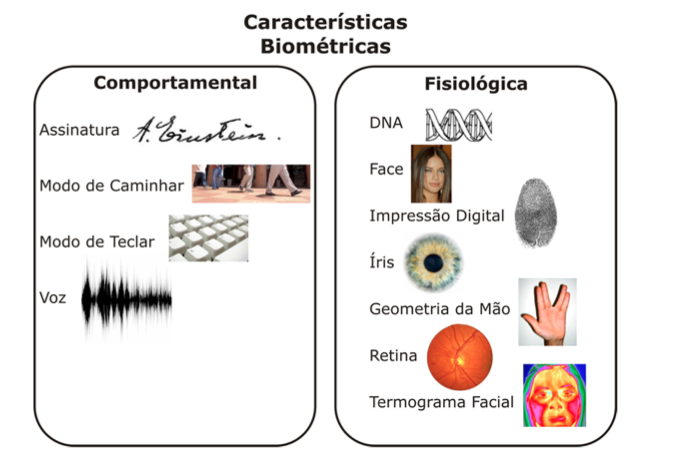
\includegraphics[scale=0.5]{figuras/2.FundamentacaoTeorica/caracteristicasBiometricas.png}
		\end{center}
		\caption{Exemplos de algumas características biométricas \cite{drovetto}.}
		\label{caracteristicasBiometricas}
	\end{figure}


	Teoricamente, qualquer característica física/comportamental pode ser utilizada
	para identificação caso siga alguns dos seguintes requisitos \cite{milene}:

	\begin{enumerate}
		\item \textbf{universalidade}: qualquer pessoa comum pode ser avaliada sobre essa característica;
		\item \textbf{singularidade}: dada duas pessoas distintas, elas não podem ter a mesma característica dentro de uma proporção satisfatória;
		\item \textbf{permanência}: a característica não pode mudar significativamente de acordo com o tempo;
		\item \textbf{exigibilidade}: pode ser mensurada quantitativamente;
	\end{enumerate}

	Porém, na prática também são considerados outros requisitos \cite{milene}:

	\begin{enumerate}
		\item \textbf{desempenho}: o processo de identificação deve apresentar um resultado aceitável;
		\item \textbf{aceitação}: indica em que ponto as pessoas estão dispostas a aceitar o sistema biométrico;
		\item \textbf{evasão}: refere-se a facilidade de ser adulterado;
	\end{enumerate}

	São várias as vantagens que os sistemas biométricos têm em relação aos sistemas
	convencionais. Listamos as vantagens principais \cite{drovetto}:
		
	\begin{itemize}
		\item características biométricas não podem ser perdidas ou esquecidas;
		\item características biométricas são difíceis de serem copiadas, compartilhadas e distribuídas;
		\item os sistemas biométricos necessitam que a pessoa esteja presente no local da autenticação;
	\end{itemize}

	Na prática um sistema biométrico deve ser capaz de \cite{hong}:
		
	\begin{enumerate}
		\item atingir uma acurácia aceitável e com uma velocidade razoável;
		\item não ser prejudicial aos indivíduos e ser aceito pela população alvo;
		\item ser suficientemente robusto para métodos fraudulentos;
	\end{enumerate}

	Novas técnicas de reconhecimento por meio de face, íris, retina e voz, entre
	outras, têm sido abordadas para aplicações em sistemas de reconhecimento
	automático \cite{bolle,saocarlos}. Das nove características utilizadas
	atualmente a face é uma das mais populares \cite{milene}. Nas Tabelas~\ref{tab:tabelaRequisitosTeoricos} e~\ref{tabelaRequisitosPraticos} são
	mostradas as noves características e seus respectivos comportamentos baseados nos requisitos
	mencionados acima.
		
	\begin{table}[h]
		\begin{center}
			\caption{Requisitos teóricos para algoritmos de reconhecimento facial \cite{milene}.}
			\label{tab:tabelaRequisitosTeoricos}
			\begin{tabular}{|c|c|c|c|c|}
				\hline \bf Biometria & \bf Universidade & \bf Singularidade & \bf Permanência & \bf Exigibilidade \\
				\hline \hline \bf Face & Alta & Baixa & Média & Alta \\
				\hline \bf  Digital & Média & Alta & Alta & Média \\
				\hline \bf Geometria da Mão & Média & Média & Média & Alta \\
				\hline \bf Veia da Mão & Média & Média & Média & Média \\
				\hline \bf Iris & Alta & Alta & Alta & Média \\
				\hline \bf Retina & Alta & Alta & Média & Baixa \\
				\hline \bf Assinatura & Baixa & Baixa & Baixa & Alta\\
				\hline \bf Voz & Média & Baixa & Baixa & Média \\
				\hline \bf Termograma & Alta & Alta & Baixa & Alta \\
				\hline
			\end{tabular}
		\end{center}
	\end{table}

	\begin{table}[h]
		\begin{center}
			\caption{Requisitos práticos para algoritmos de reconhecimento facial \cite{milene}.}
			\label{tabelaRequisitosPraticos}
			\begin{tabular}{|c|c|c|c|}
				\hline \bf Biometria & \bf Desempenho & \bf Aceitação & \bf Evasão \\
				\hline \hline \bf Face & Baixa & Alta & Baixa\\
				\hline \bf Digital & Alta & Média &  Alta\\
				\hline \bf Geometria da Mão & Média & Média & Média\\
				\hline \bf Veia da Mão & Média & Média & Alta\\
				\hline \bf Iris  & Média & Média & Alta\\
				\hline \bf Retina & Alta & Baixa & Alta\\
				\hline \bf Assinatura & Baixa & Alta & Baixa \\
				\hline \bf Voz & Baixa & Alta & Baixa \\
				\hline \bf Termograma & Média & Alta & Alta \\
				\hline
			\end{tabular}
		\end{center}
	\end{table}

	Os sistemas biométricos podem ser classificados em sistemas de verificação ou
	identificação:
	
	\begin{itemize}
		\item Sistemas de verificação são aqueles que autenticam a identidade
		dos usuários comparando-os com os próprios \textit{templates}. Eles conduzem uma
		comparação ``um para um'' e determinam se o usuário é quem realmente diz ser. O
		maior desafio para esse tipo de sistema é a acurácia. Geralmente, não é muito
		difícil satisfazer o requisito de tempo de resposta pois somente uma comparação
		``um para um'' é feita \cite{hong}.
	
		\item Sistemas de identificação reconhecem um indivíduo pesquisando em todo o
		banco de dados procurando por uma correspondência. Eles conduzem uma comparação ``um para
		muitos'' para estabelecer a identidade do indivíduo. Ao contrário dos sistemas
		de verificação, nesse tipo de sistema tanto a acurácia quanto o tempo são os
		grandes desafios, por causa da necessidade de explorar todo o banco de dados~\cite{hong}.
	\end{itemize}
	
	A face é uma característica biométrica bastante atrativa. Um dos motivos que
	incentivou os diversos estudos sobre a utilização da face para reconhecimento
	são as vantagens que ela possui em relação a impressão digital e a íris.  No
	reconhecimento por impressão digital a desvantagem consiste no fato que nem
	todas as pessoas possuem uma impressão digital com ``qualidade'' suficiente para
	ser reconhecida por um sistema. Já o reconhecimento por íris apresenta uma alta
	confiabilidade e larga variação, sendo estável pela vida toda. Porém, a
	desvantagem está relacionada ao modo de captura da íris que necessita de um
	alinhamento entre a câmera e os olhos da pessoa~\cite{saocarlos}.
	
	Além disso, aquisição da face é feita de forma fácil e não-intrusiva e possui
	uma baixa privacidade de informação, como a face é exposta constantemente, caso
	uma base de faces seja roubada, essas informações não representam algum risco e
	não possibilitam um uso impróprio.